\documentclass[11pt,a4paper]{article}

% Modèle de rapport de stage et conseils de rédaction, mise en page...
% L. Bellon, avril 2010

% définition des marges du document
\setlength{\topmargin}{0cm}
\setlength{\headheight}{0.4cm}
\setlength{\headsep}{0.8cm}
\setlength{\footskip}{1cm}
\setlength{\textwidth}{17cm}
\setlength{\textheight}{25cm}
\setlength{\voffset}{-1.5cm}
\setlength{\hoffset}{-0.5cm}
\setlength{\oddsidemargin}{0cm}
\setlength{\evensidemargin}{0cm}


% quelques package utiles
\usepackage{graphicx} % inclusion des figures

\usepackage{amsmath} % collection de symboles mathématiques
\usepackage{amssymb} % collection de symboles mathématiques
\usepackage[utf8]{inputenc}       % utilisation directe des caractères accentués sur pc
\usepackage[T1]{fontenc} % codage moderne des caractères sous Latex

\usepackage[francais]{babel}           % style français

\usepackage{tabularx} % gestion avancée des tableaux

\usepackage{psfrag} % remplacement du texte d'une figure ps par du texte latex
%\usepackage{sistyle} % mise en forme des unités

\usepackage{breqn}
\usepackage{eurosym} % symbole €
\usepackage{epstopdf} 
\def\€{\euro{}}

\usepackage{color} % gestion de différentes couleurs

\definecolor{linkcolor}{rgb}{0,0,0.6} % définition de la couleur des liens pdf
\usepackage[ pdftex,colorlinks=true,
pdfstartview=FitV,
linkcolor= linkcolor,
citecolor= linkcolor,
urlcolor= linkcolor,
hyperindex=true,
hyperfigures=false]
{hyperref} % fichiers pdf 'intelligents', avec des liens entre les références, etc.

\usepackage{fancyhdr} % entêtes et pieds de pages personnalisés

% définition de l'entête et du pied de page
\pagestyle{fancy}
\fancyhead[L]{\scriptsize \textsc{Stage M2}}
\fancyhead[R]{\scriptsize \textsc{Clément Henin}}
\fancyfoot[C]{ \thepage}

% commande d'annulation du correcteur typographique du package [francais]{babel} qui force l'espace avant ':' (parfois utile pour la bibliographie)
\makeatletter
\@ifpackageloaded{babel}%
        {\newcommand{\nospace}[1]{{\NoAutoSpaceBeforeFDP{}#1}}}%  % !! double {{}} pour cantonner l'effet à l'argument #1 !!
        {\newcommand{\nospace}[1]{#1}}
\makeatother

% commande de déplacement d'un objet
\newcommand{\drawat}[3]{\makebox[0pt][l]{\raisebox{#2}{\hspace*{#1}#3}}}

\begin{document}

% Pour faciliter la mise en forme de la page du titre, on supprime l'indentation automatique en début de paragraphe
\setlength{\parindent}{0pt}


\tableofcontents

% Première page du rapport
\setcounter{page}{1}

% on rétablit l'indentation automatique en début de paragraphe
\setlength{\parindent}{16pt}

\section{Quelques modèles liant croissance et inégalités dans les revues économiques}
\subsection{Les grands types de modèles}
\noindent
\textbf{Credit market imperfections :}\\
A cause des imperfections du marché du crédit, les pauvres peuvent avoir plus de mal à accéder au crédit. C'est le cas par exemple lorsque des lois protègent le débiteurs en défaut de paiement au détriment des créditeurs. Ces imperfections ont pour effet de diminuer les investissements de  la part des populations pauvres et par conséquent de diminuer la croissance. 

%\begin{equation}
\begin{dmath}
\text{inégalités diminuent} \implies \text{plus d'accès au crédit} \implies \text{plus d'investissements} \implies \text{la croissance augmente}
\end{dmath}
%\end{equation}

Il existe un effet inverse à ce phénomène : les coûts de lancement. Il existe des coûts irréductibles au lancement d'une entreprise/à la contraction d'un emprunt/..., il sont en proportion plus faible pour les grosses transactions. Par conséquent, une concentration des richesses induit des minimisation de ces coûts et par conséquent une augmentation de la croissance. 

\begin{dmath}
\text{inégalités diminuent} \implies \text{déconcentration des capitaux} \implies \text{investissements plus faibles} \implies \text{frais de lancement plus important} \implies \text{la croissance diminue}
\end{dmath}

Dernier effet dans cette catégorie, la présence rassurante d'un état fort et stable. La présence de ce dernier incite à accorder des crédits, on s'attend donc à ce que les effets negatifs des inégalités sur la croissance soient plus forts dans les pays pauvres que dans les pays riches. \\

\noindent
\textbf{Économie politique :}\\
L'idée sous-jacente est que nous vivons dans des démocraties. En conséquence, la majorité a la possibilité de voter pour augmenter ou diminuer les taxes. Plus précisément, si le revenu moyen dépasse le revenu médian, alors le peuple devrait voter pour des re-distributions. Ces dernières ont pour effet de diminuer l'effort au travail et par conséquent de diminuer la croissance. 

\begin{dmath}
\text{inégalités augmente} \implies \text{vote plus de redistributions} \implies \text{diminution de l'effort de travail} \implies \text{la croissance diminue}
\end{dmath}

Ces implications sont assez fausses (cf. Bénabou) : les pays les plus inégalitaires ne sont jamais ceux qui appliquent le plus de redistributions (la première implications est fausse). Il existe des modèles étudiant l'effet d'une redistribution inégale due à une répartition non-homogène du pouvoir entre les riches et le pauvres. \\

Il existe aussi un autre effet, si les riches achètent effectivement le pouvoir grâce à un lobbying puissant, cela tend à augmenter le poids de la corruption or la corruption est connue pour avoir un effet négatif sur la croissance. 

\begin{dmath}
\text{inégalités augmente} \implies \text{plus d'achat de pouvoir par les riches} \implies \text{corruption} \implies \text{la croissance diminue}
\end{dmath}

\noindent
\textbf{Agitation socio-politique :}\\
Les inégalités génèrent un sentiment d'injustice chez les pauvres. Cela augmente l'agitation sociale et crée par conséquent des pertes d'énergie conduisant à une diminution de la croissance. 

\begin{dmath}
\text{inégalités augmente} \implies \text{sentiment d'injustice} \implies \text{émeutes, crimes, révolutions} \implies \text{moins de travail} \implies \text{la croissance diminue}
\end{dmath}

\noindent
\textbf{Taux d'épargne :}\\
Le taux d'épargne augmente avec les revenus (Keyenes's General Theory). Par conséquent une société plus inégalitaire aura plus d'argent disponible pour investir et donc une croissance plus grande. 

\begin{dmath}
\text{inégalités augmente} \implies \text{plus de riches} \implies \text{épargne plus importante} \implies \text{plus d'investissement} \implies \text{la croissance augmente}
\end{dmath}

\subsection{La courbe de Kuznets - 1955}

Les liens entre le PIB/hab et les inégalités ont une forme de \og U \fg inversé.

\begin{figure}[h!]
\begin{center}
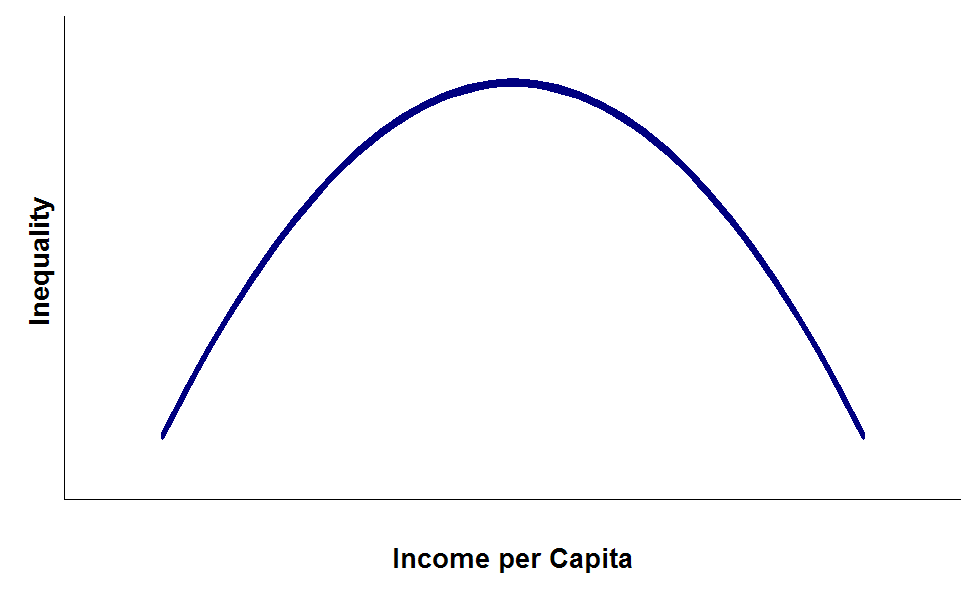
\includegraphics[scale=0.2]{Kuznets_curve.png}
\caption{Courbe de Kuznets}
\end{center}
\end{figure}

Dans la théorie de Kuznets, on suppose que la relation entre la croissance et les inégalités dépend du niveau de développement du pays : 

\begin{itemize}
\item pour les pays peu-développés, d'importants investissements dans le capital infrastructurel et naturel sont nécessaires. Ces investissements sont favorisés par une forte concentration des capitaux en faveur de ceux qui épargnent et investissent le plus. 
\item dans les économies plus avancées, les investissements conduisant à une croissance plus forte sont ceux dans le capital humain. Or cela implique une meilleure répartition des richesses afin que chacun puisse accéder à l'éducation. 
\end{itemize}

Cette courbe est largement critiquée dans \og Le Capital au XXI siècle \fg. En effet le raisonnement tel qu'il est présenté ici est incomplet. Même si dans les sociétés développées, c'est bien le capital humain qui crée de la croissance, le phénomène qui permet la redistribution des richesses n'est pas explicite. A l'inverse, comme le soutien TP, la concentration des capitaux est parfaitement stable et tend même à s'amplifier grâce à l'asymétrie des rendement des capitaux (les capitaux les plus importants obtiennent les meilleurs taux de rendement). 

\subsection{Inequality and growth in a Panel of Countries}
Barro - 2000. Utilise les données de Deininger et Squire pour mesurer les inégalités. Données concernant 84 pays. \\

\noindent
\textbf{Résumé :}\\
Dans son étude, Barro tente d'expliquer les écarts de croissance entre pays/époque grâce à un certain nombre de variables. 
\begin{equation}
Dy = F(y, y^*)
\end{equation}
Ici, $Dy$ est le taux de croissance, $y$ est le PIB/hab et $y^*$ l'ensemble des variables choisies (cf tableau \ref{barro_growth_results}). \\

Pour faire la régression, les données sont regroupées par décade : 1965 - 1975,  1975 - 1985, 1985 - 1995. Il y a donc trois points par pays et par variable. La régression est ensuite faite sur tous ces points. La dimension temporelle est donc intégrée en faisant la moyenne sur 10 ans. \\
L'auteur fait d'abord une régression linéaire sur le taux de croissance dont les résultats sont présentés dans le tableau \ref{barro_growth_results}

\begin{figure}[h!]
\begin{center}
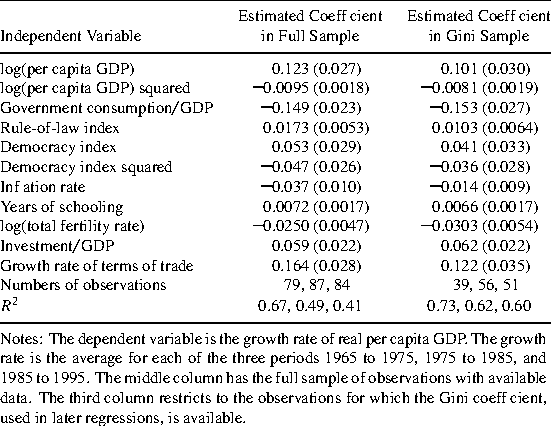
\includegraphics[scale=0.8]{barro_growth_results.pdf}
\caption{Résultats de la régression de Barro}
\label{barro_growth_results}
\end{center}
\end{figure}

Il ajoute ensuite la variable inégalités (mesurée grâce au coefficient de Gini). L'impact est nul lorsque l'on prend en compte les autres variables, il devient par exemple significatif si l'on enlève par exemple le taux de fertilité. Le résultat important vient d'une régression linéaire dont les pentes peuvent dépendre de la valeur de la variable ce qui permet d'expliquer la courbe en U inversé de Gini en fonction de GDP. Cependant, au vu de la figure présentée dans le papier (p. 19) cette régression n'a pas l'air très convaincante. \\

Les même régressions linéaires sont faites avec les quintiles pour comparer. Il trouve les mêmes résultats pour le quintile supérieur qu'avec Gini. \\
Vers la fin du papier, il utilise un indicateur mesurant l'ouverture des pays au commerce extérieur : l'ouverture d'un pays au commerce extérieure tend à augmenter les inégalités dans les pays riches (le marché du travail peu qualifié se sature) et à diminuer les inégalités dans le pays pauvres (plus de travail). \\

\noindent
\textbf{\`A tester :} \\
Si possible, récupérer les données et tracer quelques scatter plot
pour comprendre les conflits entre les variables Gini et fertilité, essayer de calculer les composantes principales des variables et voir les plus significatives -- on a des problèmes pour faire les PCA à cause des données manquantes. \\
Se renseigner sur l'indicateur de la mesure d'ouverture au commerce extérieur (p.27) pour voir s'il pourrait être intégrer à un modèle d'interaction mondiale. 

\subsection{The determinants of Economic Growth in European Regions}

Cuaresma, Doppelhofer, Feldkirchner - 2009 \\
1995 - 2005 \\
255 régions européennes \\
L'influence des inégalités n'est pas explorée. 

\noindent
\textbf{Résumé :} \\
Cette étude utilise une méthode Bayesienne pour étudier l'influence d'un grand nombre de variables sur le taux de croissance du PIB dans des régions européennes. Ils cherchent à prédire la croissance à partir de 2 types d'interactions :
\begin{itemize}
\item une régression classique sur des variables explicatives (part de la population ayant suivie des études supérieures, présence d'aéroports, présence de pôle de technologie, présence de la capital du pays, ...)
\item un terme d'interaction spatiale : il s'agit de la matrice des distances entre régions multiplié par le vecteur des taux de croissance des régions, il étudie l'influence d'une forte croissance d'une région voisine ou encore l'influence de la convergence conditionnelle des revenus. 
\end{itemize}
Les résultats de l'étude tendent à prouver que la convergence conditionnelle est le facteur le plus robuste, à noter aussi l'importance de la présence d'une capitale (qui augmente en moyenne la croissance de 1 point), la part de la population ayant suivie des études supérieures et enfin la présence d'infrastructures (notamment aéroport).\\

Le modèle utilisé est de la forme suivante : 

\begin{equation}
y = \alpha \iota_N + \rho \boldsymbol{W} y + \boldsymbol{X}_k \vec{\beta_k} + \epsilon
\end{equation}
avec $y$ un vecteur à N composantes contenant les taux de croissance de revenu par personne pour chaque région, $\iota_N$ un N-vecteur contenant des 1, $\alpha$ le terme d'interception, $\boldsymbol{X}_k = (\boldsymbol{x}_1, ..., \boldsymbol{x}_k)$ une matrice $k \times N$ contenant les $k$ variables explicatives pour chaque régions, $\boldsymbol{W}$ représente la dépendance spatiale par rapport à $y$ enfin, $\epsilon$ représente le terme d'erreur qui pourra décrire des effets spécifiques à certains pays. 

Je trouve que l'intégration d'une matrice spatial au modèle est très intéressant. L'utilisation des méthodes Bayesienne est peut-être une piste à explorer car assez visuel... 

A tester :
remplacer la matrice des distances par une matrice des echanges commerciaux (si cela existe)
mesurer la précision du modèle uniquement avec les interactions spatiales puis avec les autres variables en plus.
utiliser cette même matrice de distancec avec la variable inégalités

\subsection{A Reassessment of the Relationship Between Inequality and Growth}
Kristin J. Forbes (2000) \\
1966 - 1992 \\
45 pays  \\
(Donnes de Deininger et Squire

\noindent
\textbf{Résumé :}
Papier à contre courant du savoir actuel en 2000 qui trouve une relation positive entre inégalités des revenus et en croissance économique. Le modèle utilisé cherche une relation linéaire entre la croissance du pays i à un instant t et un ensemble de variables explicatives de ce même pays i à l'instant (t-1). 

\begin{dmath}
Growth_{i,t} = \beta_1 Inequality_{i,t - 1} + \beta_2 Income_{i,t - 1} + \beta_3 MaleEducation_{i,t - 1} + \beta_4 MaleEducation_{i,t - 1} + \beta_5 PPPI_{i, t - 1} + \alpha_i + \eta_t + u_{i,t}
\end{dmath}

Les variables utilisées sont : inégalités de revenus (Gini), les revenus, la proportion éduquée de la population (1 variable homme et une autre femme) et un mesure des distorsions due aux imperfections du marché. Plusieurs méthodes assez obscures sont utilisées, l'une d'elle est choisie comme étant la meilleure avec des arguments un peu tordus (par de mesure de précision par validation croisée par exemple). La relation positive entre les inégalités et la croissance se retrouve dans tous les modèles avec une précision importante. L'étude est ensuite comparée à celle de Perotti 1996 (qui doit être une sorte de référence) car elles obtiennent des résultats différents. Cette étude se focalise majoritairement sur les relations de court-terme entre croissance et inégalités (le temps est mesuré en période de 5 années) à la différence de l'étude de Perotti (mesure de la croissance sur longue période (30 ans) à partir de variables mesurés à l'instant initial. L'auteur fait ensuite une série de tests bizarres où il enlève des bouts de données pour tester la robustesse de ses coefficients (comme une validation croisée mais mal faite).

\begin{thebibliography}{99}

\bibitem{newmann}
  M. E. J. Newmann, 
  \emph{The structure and function of complex networks},
  Society for Industrial and Applied Mathematics
  2003.

\end{thebibliography}

\end{document}
